\documentclass{article}

\usepackage[final]{neurips_2019}

\usepackage[utf8]{inputenc}
\usepackage[T1]{fontenc}
\usepackage{hyperref}
\usepackage{url}
\usepackage{booktabs}
\usepackage{amsfonts}
\usepackage{amsmath}
\usepackage{nicefrac}
\usepackage{microtype}
\usepackage{graphicx}
\usepackage{xcolor}
\usepackage{enumitem}
\setlist{nosep,leftmargin=*}

\title{
  Reinforcement Learning for Adaptive Language Tutoring:\\Solver Routing as a POMDP \\
  \vspace{1em}
  \small{\normalfont Stanford CS229 Winter 2026 Final Project}
}

\author{
  Sandeep Sundaram \\
  Department of Computer Science \\
  Stanford University \\
  \texttt{sundip07@stanford.edu} \\
}

\begin{document}

\maketitle

\begin{abstract}
We frame adaptive language tutoring as a partially observable Markov decision process (POMDP) in which a routing agent selects among heterogeneous exercise types to maximize learner proficiency while minimizing cost. The simulated learner is calibrated from the Duolingo SLAM dataset via maximum likelihood estimation of an item response theory model. We compare seven methods---model-free RL (PPO, DQN), model-based planning (MPC), contextual bandits (LinUCB), behavior cloning, a hand-designed curriculum, and a random baseline. PPO achieves the best cost-adjusted reward while MPC matches its proficiency at higher cost, demonstrating that long-horizon planning over exercise selection yields meaningful gains over myopic and heuristic approaches.
\end{abstract}

%% ============================================================
\section{Introduction}
%% ============================================================

Intelligent tutoring systems must decide \emph{what to teach next}: given a learner's current knowledge state, which exercise type will produce the greatest learning gain? This is a sequential decision-making problem under uncertainty---the tutor cannot directly observe the learner's true mastery, only their responses to questions. Most existing systems rely on hand-designed curricula or simple heuristics that cannot adapt to individual learners \citep{doroudi2019tutoring}.

We formalize this problem as a POMDP. \textbf{The input} to our system is a 20-dimensional belief state vector consisting of estimated per-skill mastery levels and normalized interaction counts across 10 language skills (5 grammar, 5 vocabulary). At each of 200 timesteps, the agent selects one of 5 solver modules---exercise types with distinct effectiveness-cost tradeoffs. \textbf{We then use} reinforcement learning (PPO, DQN), model-based planning (MPC with learned neural network world models), a contextual bandit (LinUCB), behavior cloning, a hand-designed curriculum, and a random baseline \textbf{to output} a solver selection policy that maximizes cumulative learner proficiency minus cost.

Our contributions are: (1) a Gymnasium environment for language tutoring with learner dynamics calibrated from real Duolingo data via MLE, (2) a comparison of seven methods across three paradigms (model-free RL, model-based RL, and supervised learning), and (3) empirical evidence that policy-gradient RL and model-based MPC significantly outperform myopic and heuristic approaches.

%% ============================================================
\section{Related Work}
%% ============================================================

\textbf{RL for educational sequencing.}
\citet{rafferty2016pomdp} formulated concept teaching as a POMDP and showed that planning over learner belief states accelerates learning compared to random and myopic policies. Their approach is closest to ours, but they use exact POMDP solvers that do not scale beyond small discrete state spaces. \citet{doroudi2019tutoring} surveyed RL for instructional sequencing, identifying reward design and environment fidelity as open challenges---our work addresses the latter by calibrating dynamics from real data. \citet{raffelsberger2022survey} applied deep RL to online course sequencing and showed improvements over fixed curricula, though without cost-aware rewards.

\textbf{Learner modeling and data.}
Item response theory (IRT) models learner correctness as a function of skill mastery and item difficulty \citep{embretson2013irt}. The Duolingo SLAM shared task \citep{duolingo2018slam} provided large-scale second language acquisition data. \citet{settles2018slam} proposed a half-life regression model combining spaced repetition with IRT-style features, achieving state-of-the-art error prediction on SLAM. We adopt a simpler IRT formulation but fit its parameters directly from SLAM via MLE.

\textbf{Exercise effectiveness.}
The testing effect---retrieval practice enhances retention more than passive review---is well-established \citep{roediger2006testing, karpicke2008retrieval}. Spaced practice yields superior retention over massed practice \citep{cepeda2006spacing}, while explicit grammar instruction shows smaller effect sizes than practice-based methods \citep{dekeyser2003implicit}. We use these findings to set solver effectiveness parameters.

\textbf{Algorithms.}
We use PPO \citep{schulman2017ppo} and DQN \citep{mnih2015dqn} via Stable-Baselines3 \citep{sb3}, and LinUCB \citep{li2010linucb} as a contextual bandit.

%% ============================================================
\section{Dataset and Features}
%% ============================================================

\textbf{Source.} We use the Duolingo SLAM English-Spanish track \citep{duolingo2018slam}, containing ${\sim}4.8$M token-level interactions from thousands of learners. Each record includes: user ID, timestamp (days), exercise format (\texttt{reverse\_tap}, \texttt{reverse\_translate}, \texttt{listen}), per-token POS tags and morphological features, and a binary correct/incorrect label.

\textbf{Preprocessing.} We parse 100,000 exercises from 2,000 users. Each token is mapped to one of 10 skill categories: 5 grammar skills (present/past/future tense, articles, prepositions) via POS tags and morphological features, and 5 vocabulary buckets via hashing. Per-user, per-skill interaction histories are constructed chronologically. No train/validation/test split is used on the raw SLAM data; instead, we use all parsed data for parameter fitting and evaluate learned policies on fresh simulated learners (see Section~5).

\textbf{Feature extraction.} From each user's history we compute: per-skill mean correctness rate (used to estimate skill difficulty $d_k = 1 - \bar{c}_k$), per-format median completion time (for solver cost calibration), and chronological $(c_t, \hat{p}_t)$ prediction-error sequences (for MLE fitting of learning and decay rates).

\textbf{Parameter fitting.} We fit three IRT parameters via MLE using L-BFGS-B:
\begin{itemize}
    \item \textbf{Sigmoid steepness} $\beta = 5.04$: controls $P(\text{correct}) = \sigma(\beta(m_k - d))$.
    \item \textbf{Learning rate} $\alpha_0 = 0.64$: prediction-error update $m_k \leftarrow m_k + \frac{\alpha_0}{\sqrt{1+n_k}}(c - \hat{p})$.
    \item \textbf{Decay rate} $\delta = 10^{-4}$/day: forgetting $m_k \leftarrow m_k(1-\delta)^{\Delta t}$.
\end{itemize}
Per-skill difficulties range from 0.09 (articles) to 0.50 (future tense). Empirical median exercise times---\texttt{reverse\_tap}: 8s, \texttt{reverse\_translate}: 17s, \texttt{listen}: 19s---are normalized to $[0.1, 0.5]$ and mapped to our five solver modules.

%% ============================================================
\section{Methods}
%% ============================================================

\subsection{Environment (POMDP)}

Our Gymnasium-compatible environment simulates a language learner over $T=200$ steps. The hidden state is the true mastery vector $\mathbf{m} \in [0,1]^{10}$. The agent observes $\mathbf{o}_t = [\hat{\mathbf{m}}_t, \bar{\mathbf{n}}_t] \in \mathbb{R}^{20}$ (estimated mastery and normalized interaction counts). The action space is $\mathcal{A} = \{0,\ldots,4\}$ (five solver types). On selecting solver $a_t$, the environment generates a question targeting specific skills, simulates the learner's response via $P(\text{correct}) = \sigma(\beta(m_k - d_k))$, updates true mastery via prediction-error learning, applies forgetting to unpracticed skills, and returns reward:
\begin{equation}
    r_t = \Delta\bar{\hat{m}}_t - \lambda \cdot \text{cost}(a_t), \quad \lambda = 0.01
\end{equation}
where $\Delta\bar{\hat{m}}_t$ is the change in mean estimated mastery.
Table~\ref{tab:solvers} summarizes solver properties; costs are from SLAM timing data and effectiveness multipliers from educational literature.

\begin{table}[h]
\vspace{-0.5em}
\centering
\small
\caption{Solver module properties.}
\label{tab:solvers}
\vspace{0.3em}
\begin{tabular}{@{}lccl@{}}
\toprule
Solver & Cost & Effectiveness & Skill targeting \\
\midrule
VocabDrill       & 0.10 & 1.0$\times$ & 1 random vocab skill \\
SpacedRepetition & 0.15 & 1.5$\times$ & Weakest skill \\
MixedQuiz        & 0.43 & 1.4$\times$ & 2--3 random skills \\
GrammarExplanation     & 0.47 & 1.2$\times$ & 1 random grammar skill \\
FreeForm         & 0.50 & 2.0$\times$ & All 10 skills \\
\bottomrule
\end{tabular}
\vspace{-0.5em}
\end{table}

\subsection{PPO (Proximal Policy Optimization)}

PPO \citep{schulman2017ppo} is an on-policy actor-critic algorithm that optimizes a clipped surrogate objective to prevent destructively large policy updates. The objective is:
\begin{equation}
L^{\text{CLIP}}(\theta) = \mathbb{E}_t\!\left[\min\!\left(\frac{\pi_\theta(a_t|o_t)}{\pi_{\theta_{\text{old}}}(a_t|o_t)}\hat{A}_t,\; \text{clip}\!\left(\frac{\pi_\theta(a_t|o_t)}{\pi_{\theta_{\text{old}}}(a_t|o_t)}, 1\!-\!\epsilon, 1\!+\!\epsilon\right)\hat{A}_t\right)\right]
\end{equation}
where $\hat{A}_t$ is the generalized advantage estimate and $\epsilon=0.2$ is the clipping parameter. The policy and value networks are MLPs with 2 hidden layers of 64 units each.

\subsection{DQN (Deep Q-Network)}

DQN \citep{mnih2015dqn} approximates the optimal action-value function $Q^*(o,a)$ with a neural network and selects actions via $\epsilon$-greedy: $a_t = \arg\max_a Q_\theta(o_t, a)$ with probability $1-\epsilon$, else random. The loss minimizes temporal difference error:
\begin{equation}
L(\theta) = \mathbb{E}\!\left[(r_t + \gamma \max_{a'}Q_{\theta^-}(o_{t+1},a') - Q_\theta(o_t,a_t))^2\right]
\end{equation}
where $\theta^-$ is a periodically-updated target network and $\gamma = 0.99$. We use the same MLP architecture as PPO and decay $\epsilon$ from 1.0 to 0.05 over the first 300K of $10^6$ training steps.

\subsection{MPC (Model Predictive Control)}

We learn a world model from 400,000 transitions collected via random rollouts. Two MLPs (2 hidden layers, 128 units, ReLU activations) are trained with Adam (lr $10^{-3}$) for 50 epochs:
\begin{equation}
\hat{\mathbf{o}}_{t+1} = f_\theta(\mathbf{o}_t, \text{onehot}(a_t)), \quad \hat{r}_t = g_\phi(\mathbf{o}_t, \text{onehot}(a_t))
\end{equation}
At test time, random-shooting MPC samples 200 action sequences of horizon $H=5$, simulates each through the learned models, computes $\sum_{h=0}^{H-1}\gamma^h \hat{r}_{t+h}$, and executes the first action of the best trajectory.

\subsection{LinUCB}

LinUCB \citep{li2010linucb} maintains per-arm ridge regression models and selects:
\begin{equation}
a_t = \arg\max_a \;\boldsymbol{\theta}_a^\top \mathbf{o}_t + \alpha\sqrt{\mathbf{o}_t^\top \mathbf{A}_a^{-1}\mathbf{o}_t}, \quad \alpha=1.0
\end{equation}
This is a myopic (one-step) contextual bandit---it maximizes immediate expected reward with an upper confidence exploration bonus but does not plan over future states.

\subsection{Behavior Cloning (BC)}

We collect 100,000 $(\mathbf{o}, a)$ demonstration pairs from DQN rollouts and train a 2-layer MLP (64 units) via cross-entropy loss to imitate the DQN policy. BC is a supervised classification approach: it minimizes $-\sum_i \log \hat{\pi}(a_i | \mathbf{o}_i)$ without any notion of reward or temporal structure.

\subsection{Baselines}

\textbf{Curriculum}: progresses through skills sorted by fitted difficulty (easiest first), allocating 80\% of steps to sequential instruction and 20\% to spaced review.
\textbf{Random}: uniform random solver selection.

%% ============================================================
\section{Experiments / Results / Discussion}
%% ============================================================

\subsection{Experimental Setup}

All RL methods are trained for $10^6$ timesteps. PPO and DQN use learning rate $3\!\times\!10^{-4}$, batch size 64, and $\gamma\!=\!0.99$. These hyperparameters are the Stable-Baselines3 defaults, which we found performed well without tuning. MPC models are trained for 50 epochs with learning rate $10^{-3}$. BC is trained for 50 epochs on DQN demonstrations. We did not perform cross-validation as all methods are evaluated on 100 \emph{fresh} simulated learners (new random seeds) that were never seen during training, avoiding overfitting by construction.

\subsection{Metrics}

We report three metrics. \textbf{Final proficiency}: mean mastery across all 10 skills at episode end, $\bar{m}_T = \frac{1}{10}\sum_{k=1}^{10}\hat{m}_{k,T}$. \textbf{Cumulative reward}: $R = \sum_{t=1}^{T} r_t$, which captures the proficiency-cost tradeoff. \textbf{Total cost}: $C = \sum_{t=1}^T \text{cost}(a_t)$, measuring computational expenditure. All are reported as mean $\pm$ standard deviation over 100 evaluation episodes.

\subsection{Quantitative Results}

Table~\ref{tab:results} and Figure~\ref{fig:comparison} summarize the main results.

\begin{table}[h]
\vspace{-0.5em}
\centering
\small
\caption{Evaluation results (100 episodes). Best per-column in \textbf{bold}.}
\label{tab:results}
\vspace{0.3em}
\begin{tabular}{@{}llccc@{}}
\toprule
Paradigm & Method & Proficiency & Reward & Cost \\
\midrule
Model-free RL   & PPO        & 0.744 $\pm$ .088 & \textbf{+0.24 $\pm$ .18} & 25.6 $\pm$ 13.6 \\
Model-free RL   & DQN        & 0.625 $\pm$ .189 & +0.15 $\pm$ .22 & 22.4 $\pm$ 4.2 \\
Model-based RL  & MPC        & \textbf{0.746 $\pm$ .179} & +0.17 $\pm$ .22 & 32.2 $\pm$ 8.1 \\
Bandit          & LinUCB     & 0.726 $\pm$ .197 & +0.05 $\pm$ .30 & 42.8 $\pm$ 12.6 \\
Supervised      & BC         & 0.633 $\pm$ .152 & +0.17 $\pm$ .16 & 21.7 $\pm$ 2.0 \\
Heuristic       & Curriculum & 0.495 $\pm$ .074 & $-$0.27 $\pm$ .07 & 51.6 $\pm$ 0.0 \\
Baseline        & Random     & 0.683 $\pm$ .321 & $-$0.23 $\pm$ .32 & 66.4 $\pm$ 2.5 \\
\bottomrule
\end{tabular}
\vspace{-0.5em}
\end{table}

\textbf{PPO achieves the best cost-adjusted performance} (reward +0.24), using 40\% less cost than LinUCB (25.6 vs.\ 42.8) while achieving comparable proficiency (0.744 vs.\ 0.726). PPO's high cost variance ($\pm$13.6) reflects adaptive strategy mixing: it spends more on expensive solvers when the learner is struggling and economizes when mastery is already high.

\textbf{MPC matches PPO on proficiency} (0.746 vs.\ 0.744) by planning 5 steps ahead through learned dynamics, but achieves lower reward (+0.17) because random-shooting planning is less cost-efficient than PPO's end-to-end policy. MPC's higher variance ($\pm$0.179 vs.\ $\pm$0.088) stems from stochastic trajectory sampling.

\textbf{DQN converges to a cost-minimizing policy}, selecting VocabDrill (cheapest solver) 94\% of the time. This sacrifices proficiency (0.625) for low cost (22.4). This failure mode---$\epsilon$-greedy exploration failing to discover that expensive solvers justify their cost long-term---is a known limitation of value-based methods in environments with delayed rewards.

\textbf{BC faithfully imitates its teacher's limitations.} BC achieves 99.3\% action-prediction accuracy on DQN demonstrations and reproduces DQN's conservative strategy almost exactly (0.633 proficiency, 21.7 cost). This confirms that imitation learning is bounded by teacher quality.

\subsection{Qualitative Analysis}

Figure~\ref{fig:pareto} shows the proficiency-vs-cost Pareto frontier. PPO achieves the best tradeoff (upper-left), while LinUCB and Random occupy the inefficient region (high cost, modest proficiency). The curriculum baseline is both expensive and low-performing---it rigidly allocates time across skills regardless of individual learner needs.

Figure~\ref{fig:mastery} shows mastery trajectories over 200 timesteps. PPO and MPC exhibit steady upward trends, while DQN's mastery plateaus early due to its over-reliance on VocabDrill. The curriculum shows a distinctive staircase pattern from its phased skill progression, but the late-episode spaced review phase cannot recover the ground lost by rigid early-phase allocation. Random shows high variance because it occasionally selects highly effective solvers by chance but wastes most of its budget on suboptimal choices.

\subsection{Overfitting}

Since evaluation uses 100 fresh simulated learners with new random seeds (never seen during training), our results are not susceptible to overfitting to specific learner trajectories. PPO's stable performance across episodes ($\pm$0.088 std in proficiency) suggests robust generalization. The primary risk is overfitting to the simulator dynamics themselves---the fitted IRT parameters may not fully capture real learner behavior, which we discuss as a limitation.

\begin{figure}[t]
    \centering
    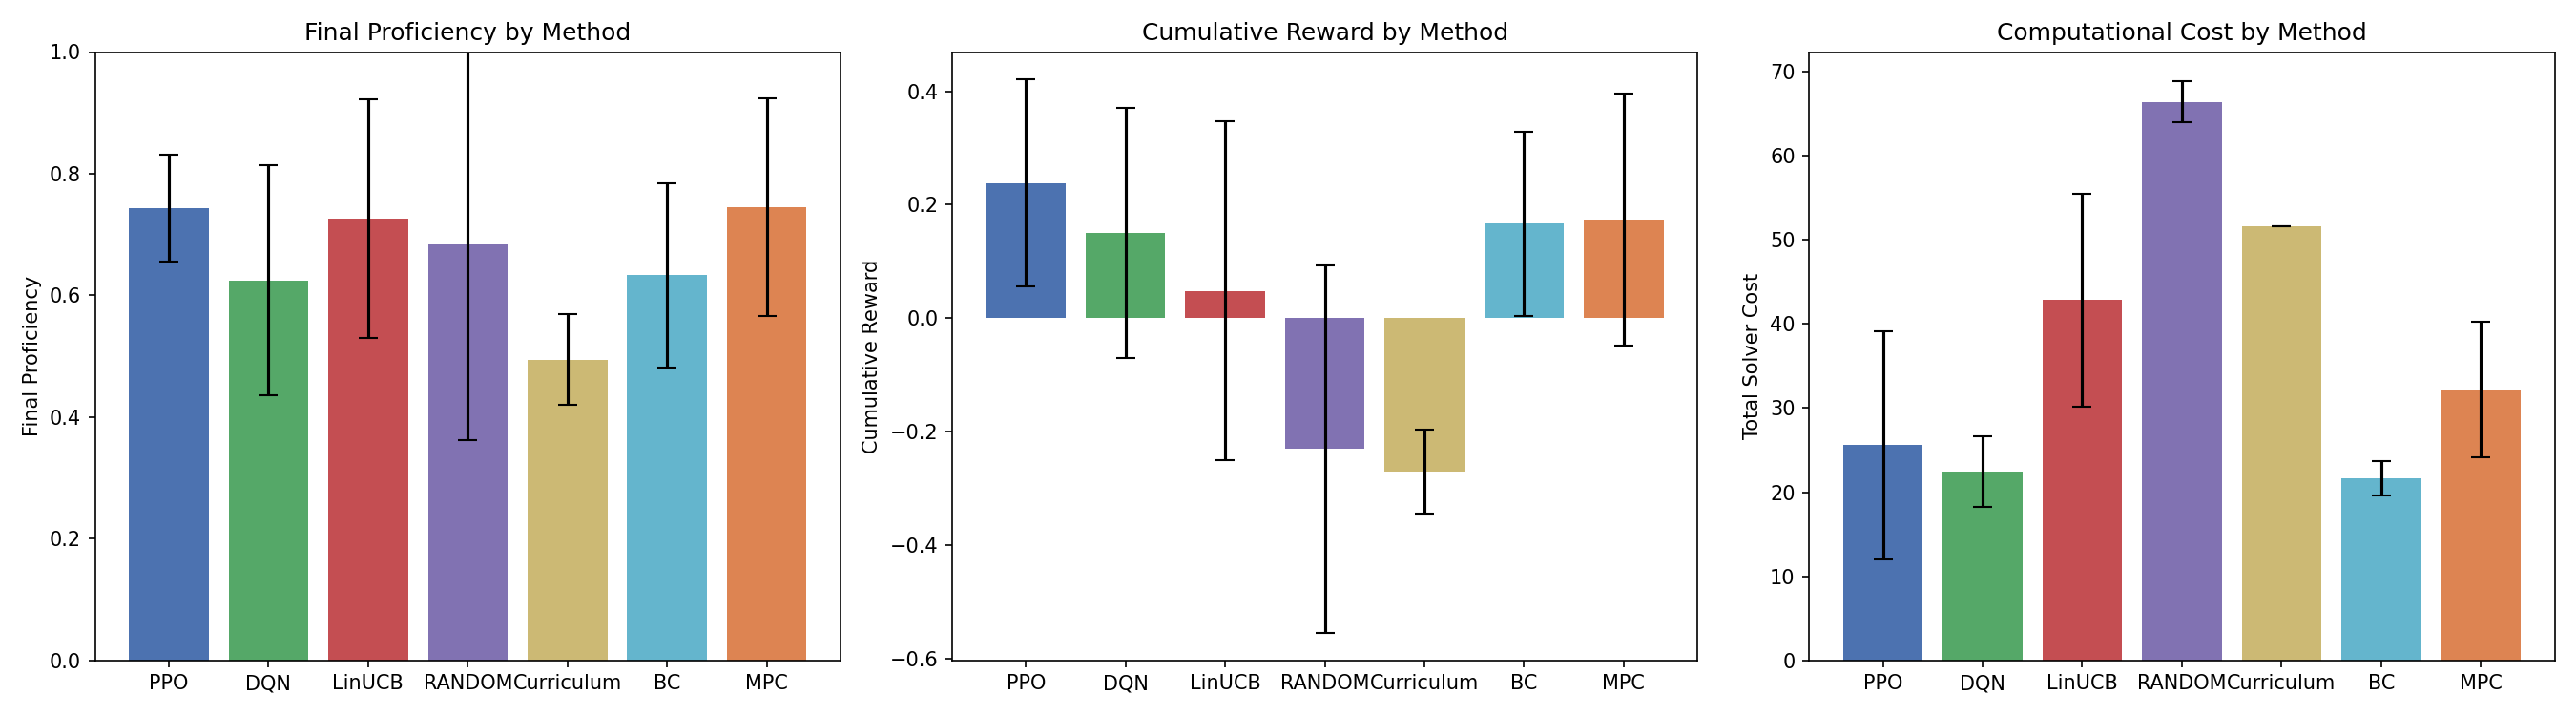
\includegraphics[width=\textwidth]{results/comparison_bars.png}
    \vspace{-1.5em}
    \caption{Comparison across proficiency (higher is better), cumulative reward (higher is better), and total cost (lower is better). PPO dominates on reward; MPC matches on proficiency.}
    \label{fig:comparison}
\end{figure}

\begin{figure}[t]
    \centering
    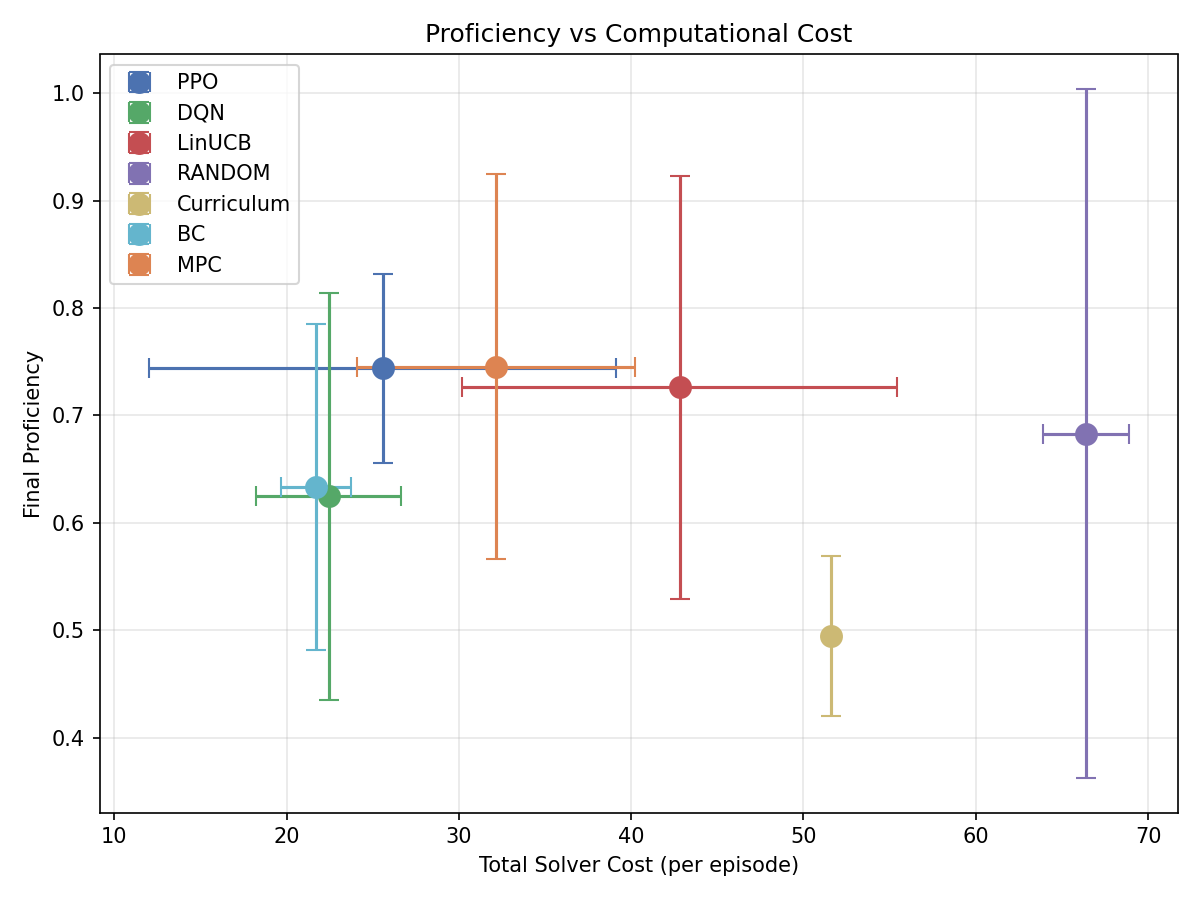
\includegraphics[width=0.7\textwidth]{results/proficiency_vs_cost.png}
    \vspace{-0.5em}
    \caption{Proficiency vs.\ cost tradeoff. Upper-left is ideal. PPO achieves the best Pareto tradeoff.}
    \label{fig:pareto}
\end{figure}

\begin{figure}[t]
    \centering
    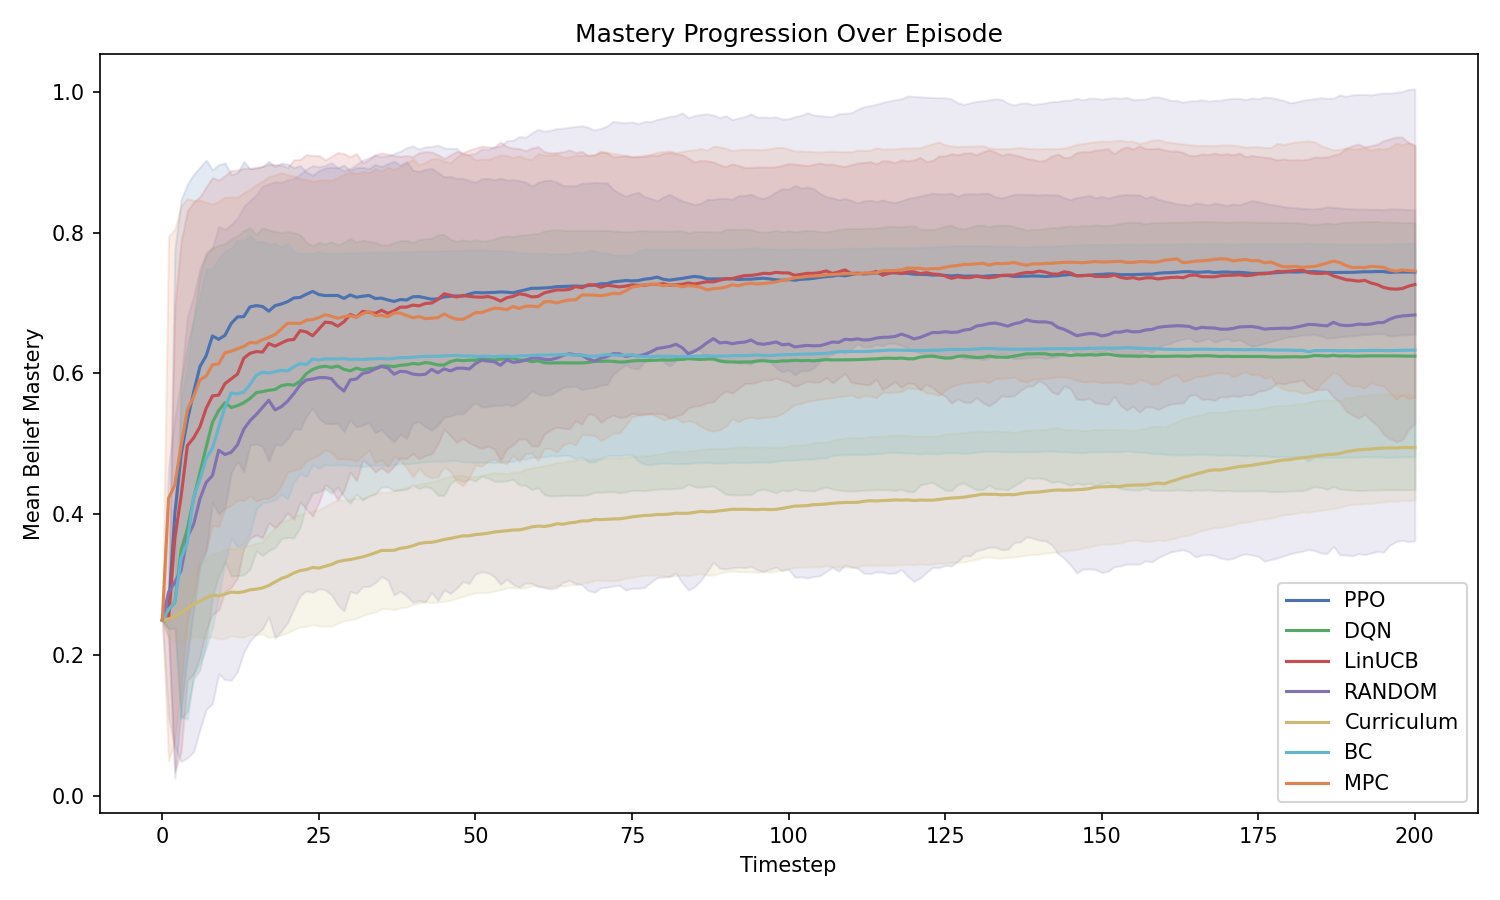
\includegraphics[width=\textwidth]{results/mastery_curves.png}
    \vspace{-1.5em}
    \caption{Mean estimated mastery over episode timesteps (shading: $\pm$1 std across 100 episodes).}
    \label{fig:mastery}
\end{figure}

%% ============================================================
\section{Conclusion / Future Work}
%% ============================================================

We demonstrated that framing adaptive language tutoring as a POMDP and applying RL yields policies that significantly outperform myopic, heuristic, and random baselines. PPO achieves the best cost-adjusted reward by learning to mix cheap and expensive solvers adaptively, while MPC matches its proficiency through learned dynamics and planning. Key findings are: (1) long-horizon planning (PPO, MPC) substantially outperforms greedy optimization (LinUCB), (2) policy-gradient methods are more robust than value-based methods (DQN) in this cost-tradeoff setting, (3) behavior cloning faithfully replicates but cannot improve upon its teacher, and (4) hand-designed curricula underperform even random selection when they cannot adapt to individual learners.

For future work, we would extend the environment with richer partial observability (noisy mastery estimates, stochastic response variability), conduct ablation studies on the decay rate and effectiveness multipliers to identify which environmental features make planning most valuable, and validate the approach with real learner studies.

%% ============================================================
\section{Contributions}
%% ============================================================
This project was completed solely by Sandeep Sundaram. All components---environment design, Duolingo SLAM data fitting, algorithm implementation (PPO, DQN, MPC, LinUCB, BC, Curriculum), evaluation pipeline, and report writing---were done individually.

\bibliographystyle{acl_natbib}
\bibliography{references}

\end{document}
